
Our claim is that feedback volume is inversely related to repair utility, and that the lightest verifier --- not the most informative one --- wins on correctness per second. We build to it in the order the experiments depend on each other: first that the comparison is well-posed, then that the categories genuinely differ, then the inversion, then the cost reversal.

\subsubsection{5.1 The Comparison Is Well-Posed (RQ1)}

Figure 1 reports verifier activation across all 421 problems. Execution monitoring, static analysis, and type checking each fire on 100\% of GPT-4o-mini completions, far above the 10\% threshold set as the minimum for a category to be worth comparing. SMT solving fires on none.

\begin{figure}[htbp]
\centering
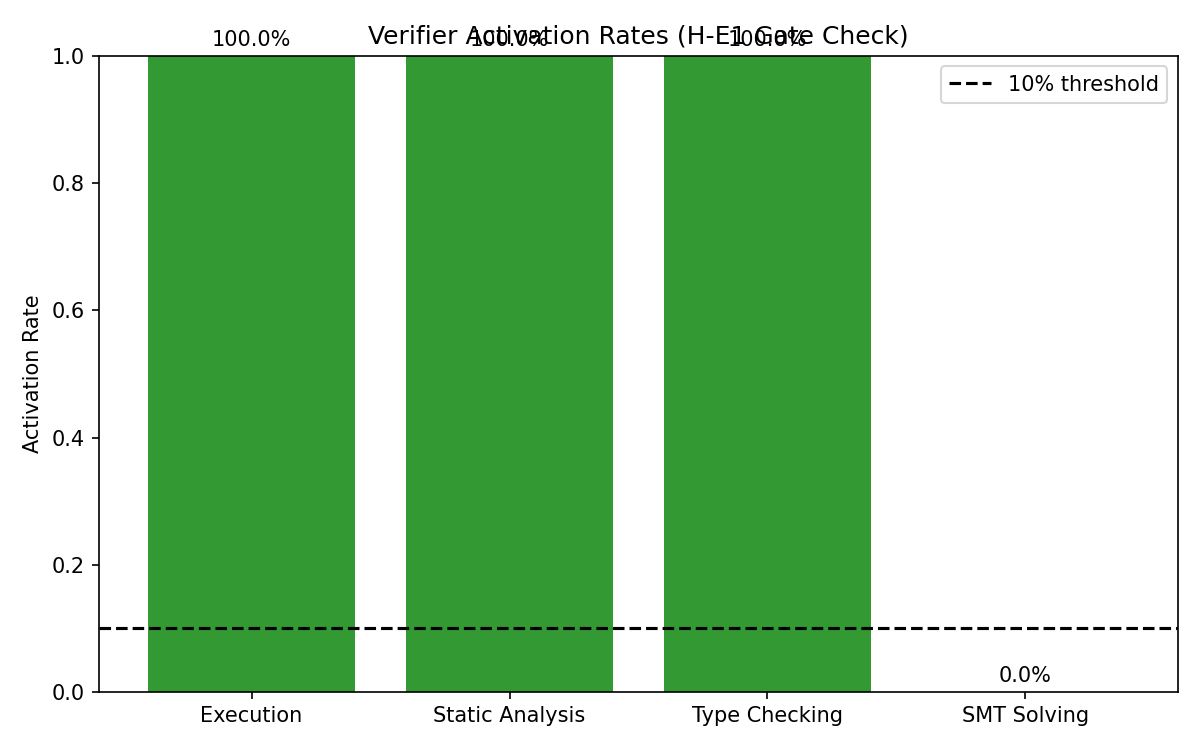
\includegraphics[width=\columnwidth]{figures/activation_rates.png}
\caption{Verifier activation rates}
\label{fig:activation_rates}
\end{figure}

\textbf{Figure 1:} Activation rate per feedback category over 421 HumanEval and MBPP problems. Three categories fire universally; SMT is disabled after its pilot.

Two things follow. First, any difference in downstream repair cannot be attributed to one category simply having nothing to say --- all three active verifiers produce output on every problem. Second, the universal activation is itself a comment on single-shot LLM code: a completion that triggers the execution verifier also triggers the type checker and the static analyzer, essentially always. Whatever complementarity they have must live in the content of what they report.

The SMT result is a different kind of finding. A 20-problem pilot produced 0 SAT outcomes (Figure 2), against the roughly 40\% constraint coverage our design assumed. GPT-4o-mini could not reliably translate HumanEval's informal docstrings into valid Z3 constraints, and we scoped the primary comparison to three categories as a result.

\begin{figure}[htbp]
\centering
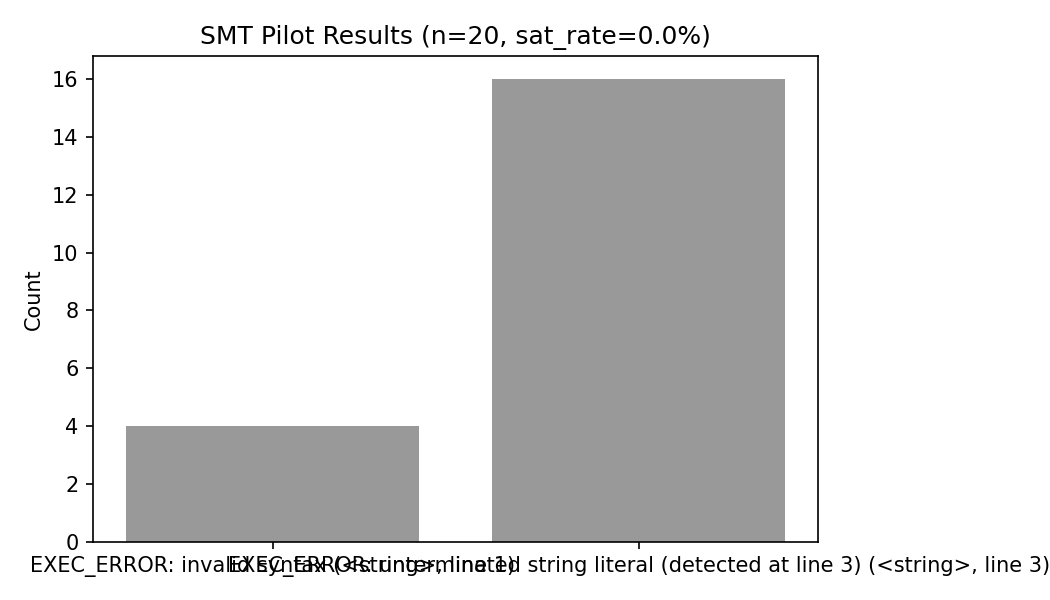
\includegraphics[width=\columnwidth]{figures/smt_pilot.png}
\caption{SMT pilot results}
\label{fig:smt_pilot}
\end{figure}

\textbf{Figure 2:} SMT constraint-extraction pilot. Zero of 20 sampled problems yielded a SAT outcome from model-generated Z3 constraints.

\subsubsection{5.2 What Has to Be Repaired (RQ2)}

GPT-4o-mini solves 70.1\% of the 421 problems on the first attempt --- 86.0\% of HumanEval (141/164 passing), 59.9\% of MBPP (154/257 passing) --- leaving 126 failures. Figure 3 shows how they distribute.

\begin{figure}[htbp]
\centering
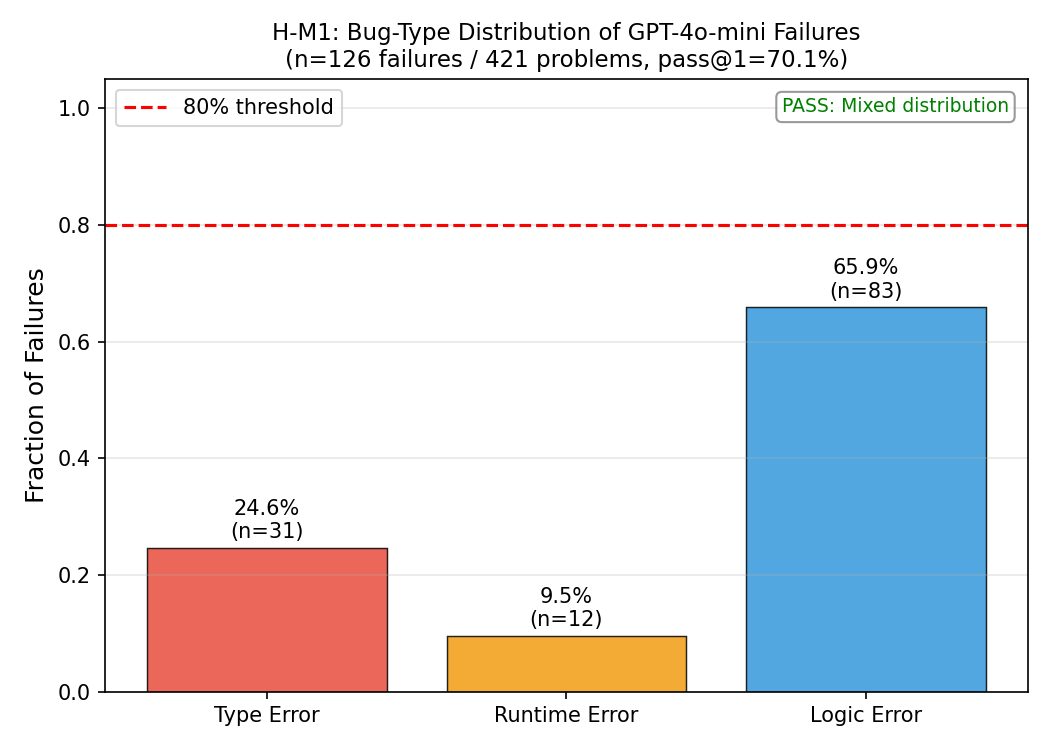
\includegraphics[width=\columnwidth]{figures/bug_distribution.png}
\caption{Bug type distribution}
\label{fig:bug_distribution}
\end{figure}

\textbf{Figure 3:} Bug-type distribution over 126 failing solutions. Logic errors 65.9\%, type errors 24.6\%, runtime errors 9.5\%.

\begin{table}[htbp]
\centering
\resizebox{\columnwidth}{!}{%
\begin{tabular}{lll}
\toprule
Bug type & Count & Fraction \\
\midrule
Logic error & 83 & 65.9\% \\
Type error & 31 & 24.6\% \\
Runtime error & 12 & 9.5\% \\
\bottomrule
\end{tabular}
}
\end{table}

No single type exceeds 80\%, so the comparison has something to discriminate. A spot check of 50 classifications against manual labels agreed 82\% of the time, above the 70\% reliability threshold.

The composition matters more than the mixedness. Two thirds of failures are logic errors --- code that parses cleanly, type-checks, runs to completion without raising, and returns the wrong answer. This population is largely invisible to static tooling by construction: a type checker cannot see that a sorting function sorts in the wrong direction. That observation alone predicts a ceiling on how much static analysis can contribute to absolute correctness.

Figure 4 splits the distribution by benchmark. HumanEval's 23 failures are predominantly logic errors (15/23 logic, 5/23 type, 3/23 runtime); MBPP's 103 split 66\% logic (68), 25\% type (26), 9\% runtime (9).

\begin{figure}[htbp]
\centering
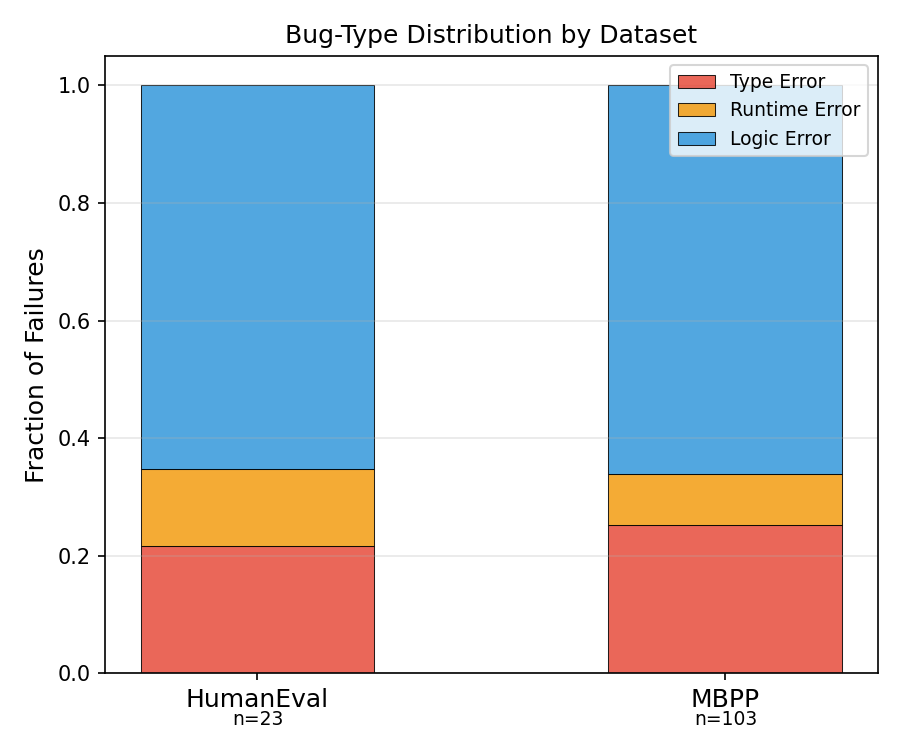
\includegraphics[width=\columnwidth]{figures/stacked_by_dataset.png}
\caption{Bug types by dataset}
\label{fig:stacked_by_dataset}
\end{figure}

\textbf{Figure 4:} Bug-type composition by benchmark.

\subsubsection{5.3 The Categories Differ Enormously (RQ3)}

Applying all four verifiers to the same 126 failing solutions produces feedback volumes separated by four orders of magnitude.

\begin{table*}[htbp]
\centering
\resizebox{\dimexpr 2\columnwidth+\columnsep\relax}{!}{%
\begin{tabular}{lllll}
\toprule
Verifier & Mean chars & Median & Std & n \\
\midrule
Pyright (static) & 24,358.7 & 27,755.0 & 12,162.8 & 126 \\
Execution & 201.8 & 166.5 & 84.7 & 126 \\
mypy (type) & 48.7 & 55.0 & 23.4 & 126 \\
Z3 (SMT) & 2.0 & 2.0 & 0.0 & 8 \\
\bottomrule
\end{tabular}
}
\end{table*}

Kruskal-Wallis confirms the differences are not noise: H = 338.78, p = 4.$01\times 10^{-73}, \epsilon ^2$ = 0.880 --- a very large effect. All pairwise Dunn comparisons are significant under Bonferroni correction except mypy versus Z3, where both means sit near zero. Z3 coverage was 6.3\% (8/126 problems yielded constraints).

\begin{figure}[htbp]
\centering
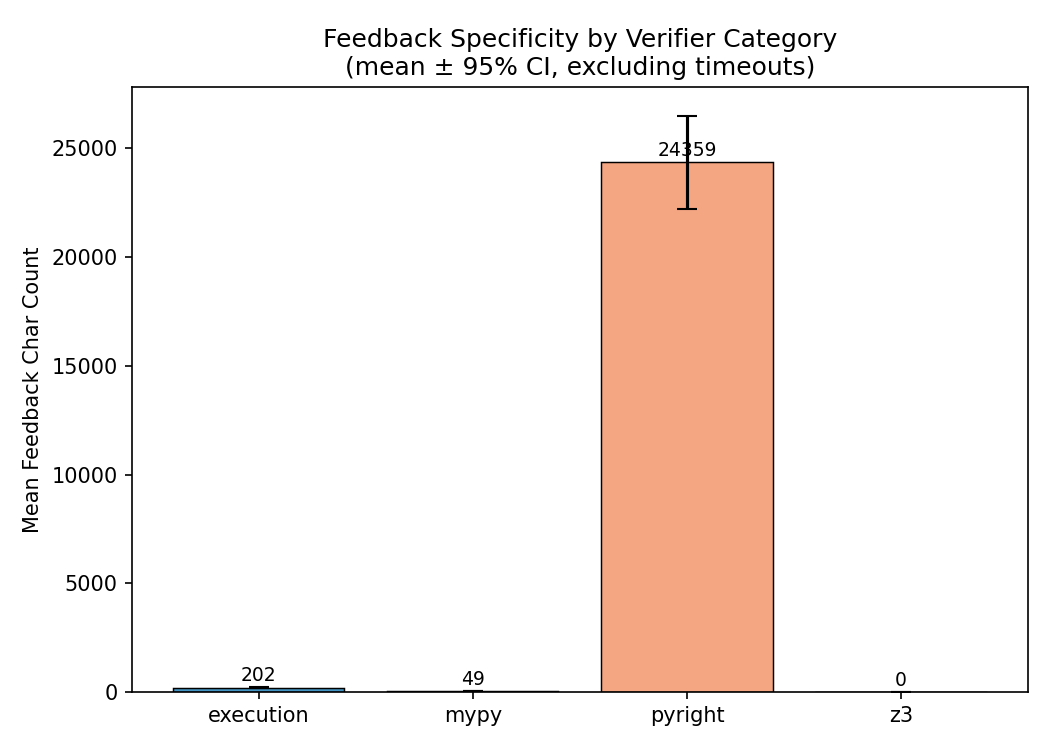
\includegraphics[width=\columnwidth]{figures/bar_mean_char_count.png}
\caption{Mean feedback length}
\label{fig:bar_mean_char_count}
\end{figure}

\textbf{Figure 5:} Mean feedback character count per verifier with 95\% confidence intervals.

\begin{figure}[htbp]
\centering
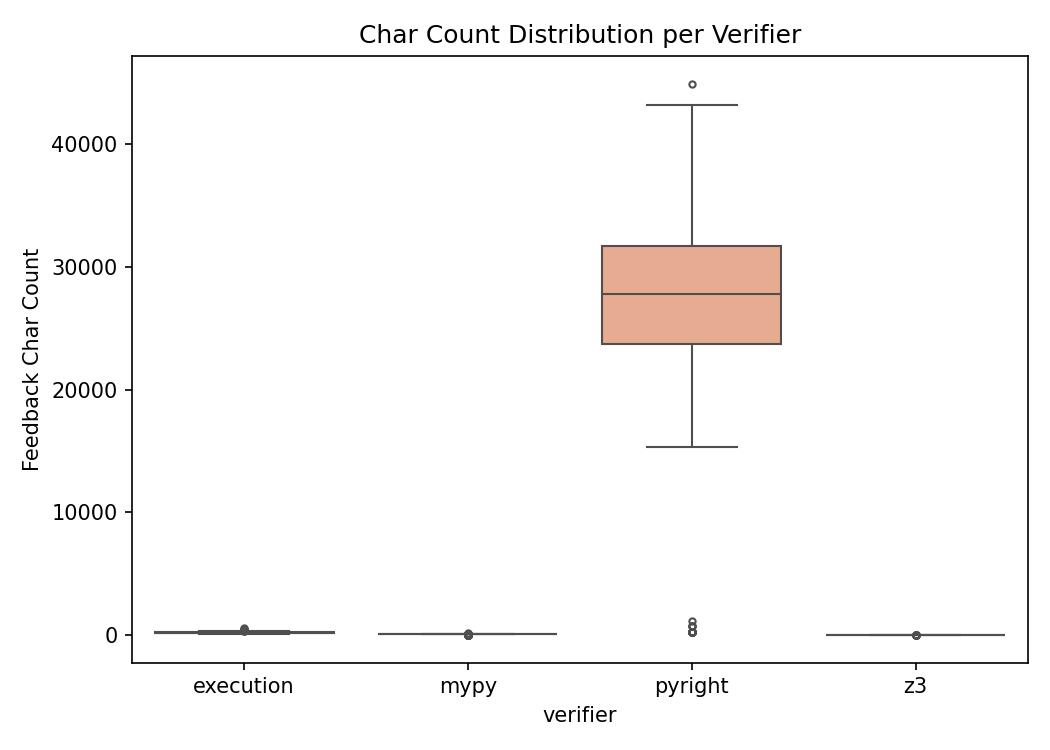
\includegraphics[width=\columnwidth]{figures/box_char_count.png}
\caption{Feedback length distributions}
\label{fig:box_char_count}
\end{figure}

\textbf{Figure 6:} Per-verifier feedback length distributions (log scale).

The observed ordering is Pyright ≫ execution > mypy ≫ Z3, which is not the ordering the specificity intuition predicts. We expected SMT at the top; instead the top slot goes to Pyright, and for a reason that has little to do with formal precision: its JSON diagnostic record serializes the full analysis, including unused-import notices and missing-annotation warnings alongside anything relevant to the failing test. mypy sits near the bottom because LLM-generated Python carries almost no type annotations. Z3 sits at the bottom on 8 problems because it emits a two-character sentinel when it has anything to say at all. This establishes that the independent variable has real range.

\subsubsection{5.4 The Inversion (RQ4)}

Feeding each category's feedback into the repair loop over the same 126 failing solutions produces the paper's central result.

\begin{table*}[htbp]
\centering
\resizebox{\dimexpr 2\columnwidth+\columnsep\relax}{!}{%
\begin{tabular}{lllll}
\toprule
Verifier & Specificity rank (by char count) & Iteration-1 repair rate & 95\% CI & Mean iters to pass \\
\midrule
Pyright (static) & 1 (most verbose) & 4.76\% & [1.6\%, 8.7\%] & 1.375 \\
Execution & 2 & 5.56\% & [1.6\%, 9.5\%] & 1.727 \\
mypy (type) & 3 & 6.35\% & [2.4\%, 11.1\%] & 1.455 \\
Z3 (SMT) & 4 (least verbose) & 7.94\% & [4.0\%, 12.7\%] & 1.167 \\
\bottomrule
\end{tabular}
}
\end{table*}

The repair rate falls monotonically as feedback volume rises. Spearman's $\rho$ over the four categories is \textbf{-1.0000} --- a perfect inverse rank correlation. The relationship holds when Z3 is dropped ($\rho$ = -1.0 over the remaining three categories), at iteration 2 ($\rho$ = -0.800), and within every bug-type stratum examined (logic $\rho$ = -0.949, type $\rho$ = -0.894, runtime $\rho$ = -0.775).

\begin{figure}[htbp]
\centering
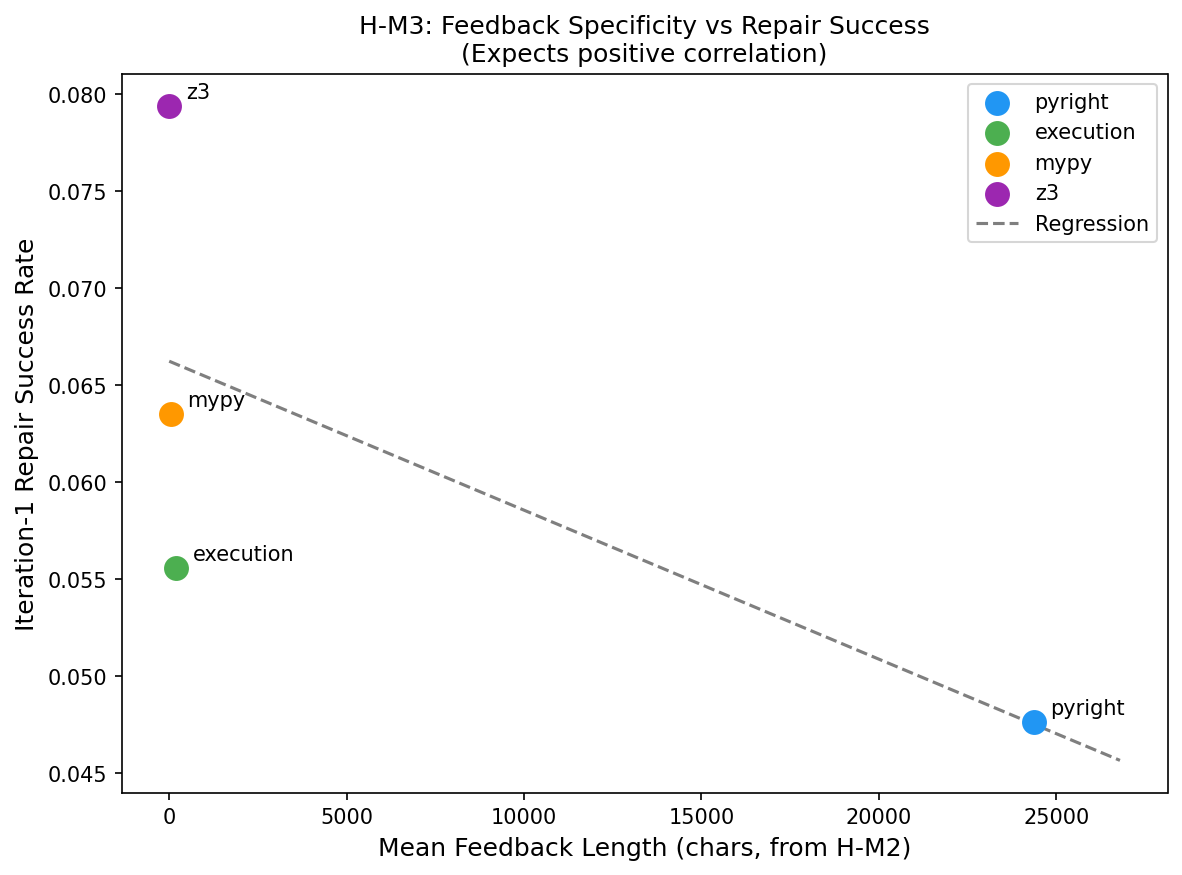
\includegraphics[width=\columnwidth]{figures/scatter_length_vs_rate.png}
\caption{Feedback length versus repair rate}
\label{fig:scatter_length_vs_rate}
\end{figure}

\textbf{Figure 7:} Mean feedback length against iteration-1 repair rate. The relationship is perfectly monotone and negative ($\rho$ = -1.0).

\begin{figure}[htbp]
\centering
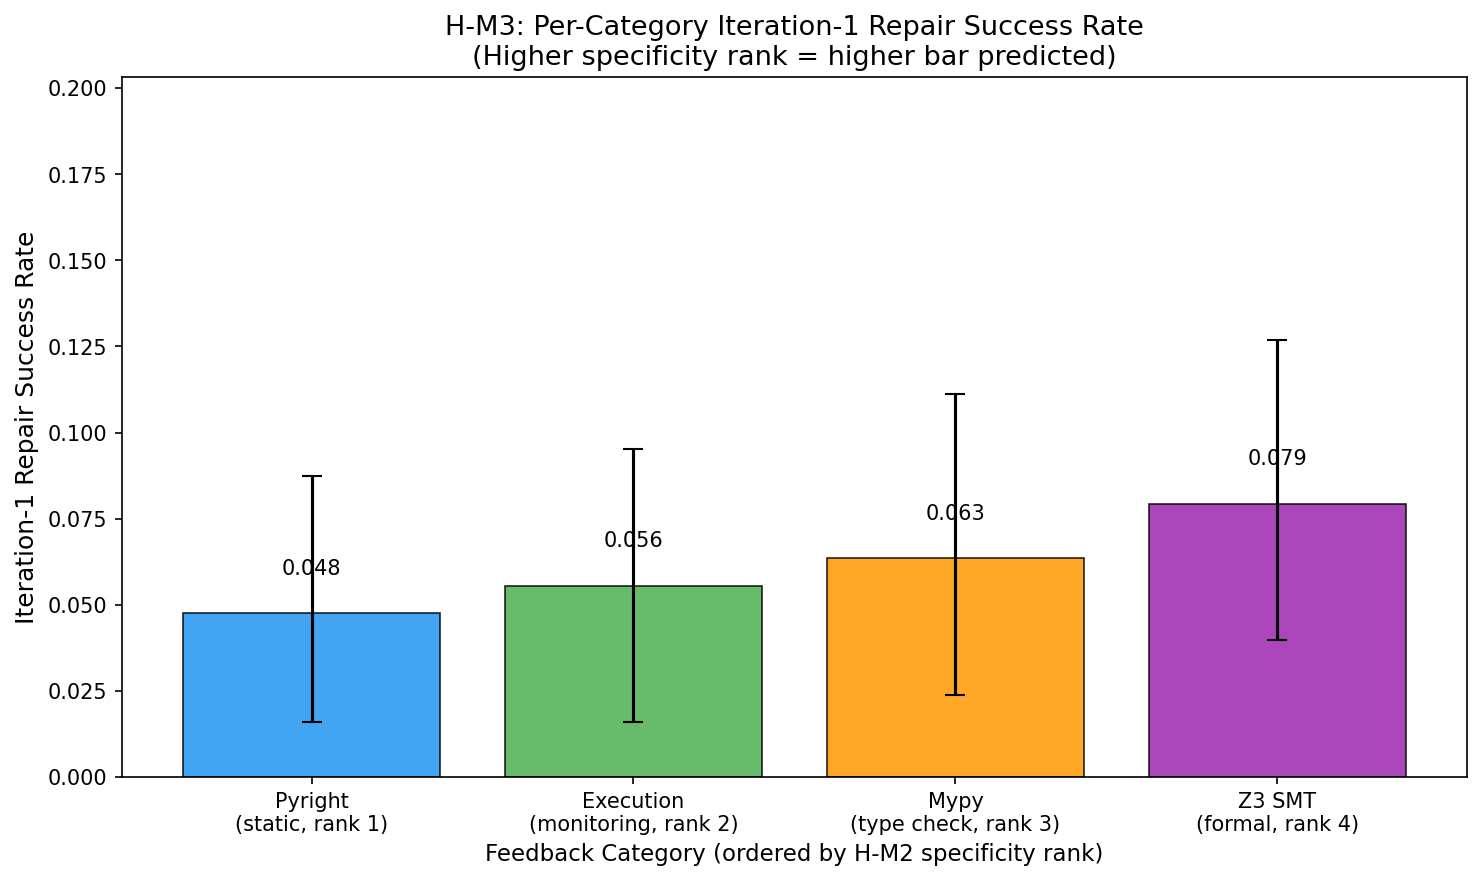
\includegraphics[width=\columnwidth]{figures/bar_iter1_rate.png}
\caption{Iteration-1 repair rates}
\label{fig:bar_iter1_rate}
\end{figure}

\textbf{Figure 8:} Iteration-1 repair rate per category with bootstrap 95\% confidence intervals (n = 126).

We had predicted $\rho$ > 0 and pre-registered that as the gate condition. We got $\rho$ = -1.0, which fails the gate in the most complete way available.

Two cautions belong here before any interpretation. The confidence intervals overlap substantially --- the categories are separated by a few percentage points on 126 problems, and no single pairwise difference is individually significant. What is striking is not the size of any gap but the perfect monotonicity of the ordering across four categories, which persists under every stratification attempted. And $\rho$ computed over four points is a coarse statistic; it can only take a handful of values, and -1.0 means ''perfectly ordered,'' not ''strongly correlated'' in the usual sense.

With those caveats, the direction is clear and it is the opposite of what the field assumes. Our reading, developed in Section 6, is that repair is bounded by the model's ability to extract one actionable edit from the feedback rather than by the feedback's information content --- a 202-character traceback naming a line and an exception type is actionable on sight, while 4,000 characters of surviving JSON require the model to first identify which of forty diagnostics broke the test.

Figure 9 tracks cumulative repair across the full three-iteration budget. The gaps narrow but the ordering does not reverse.

\begin{figure}[htbp]
\centering
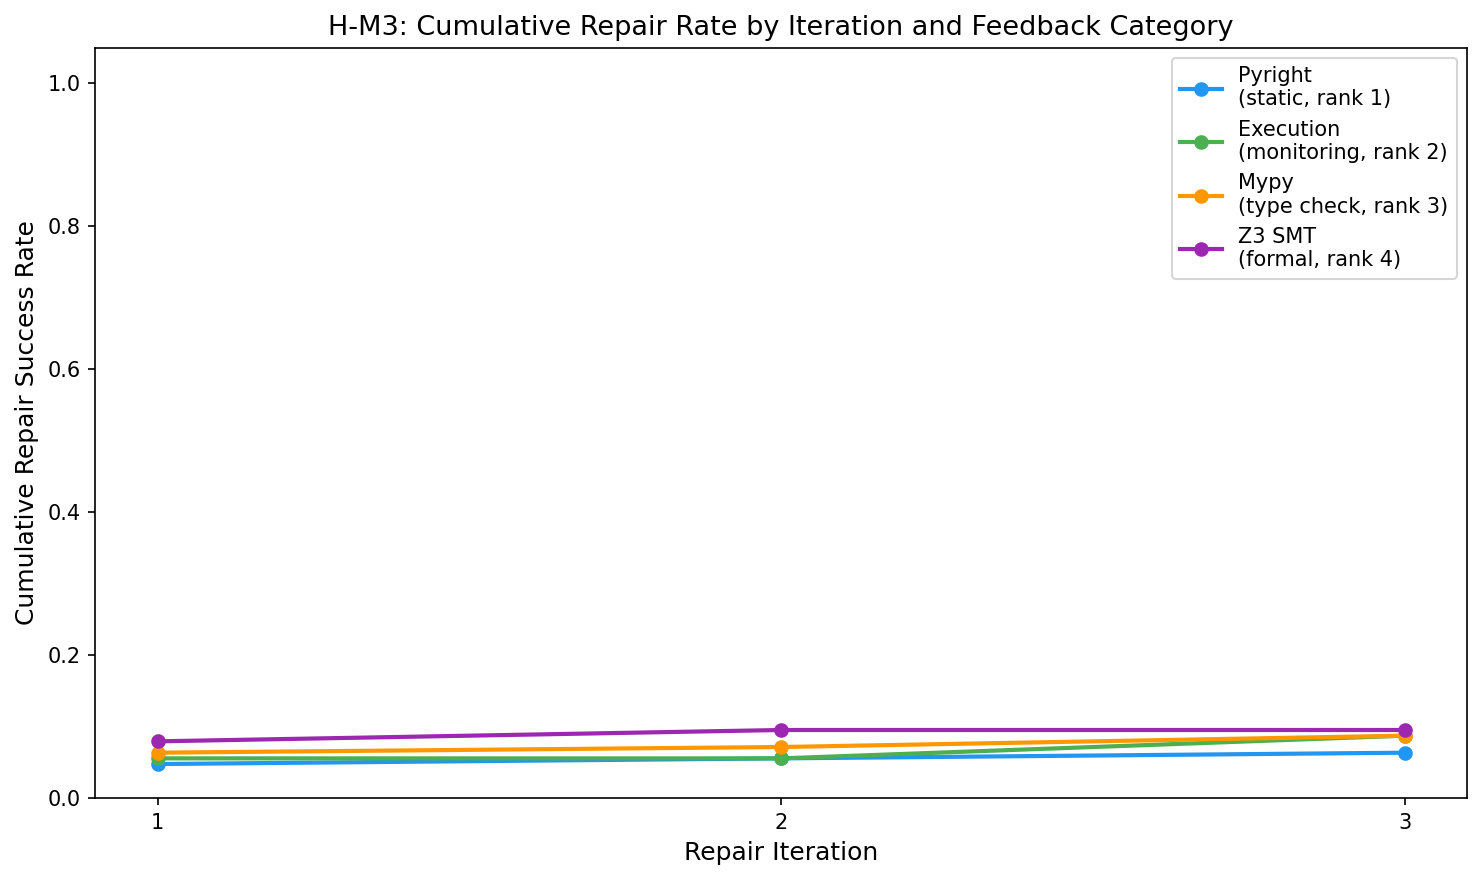
\includegraphics[width=\columnwidth]{figures/line_cumulative_repair.png}
\caption{Cumulative repair across iterations}
\label{fig:line_cumulative_repair}
\end{figure}

\textbf{Figure 9:} Cumulative repair rate across the three-iteration budget.

One detail cuts against the simplest reading: Pyright has the \textit{lowest} mean iterations-to-pass among the active verifiers at 1.375. When Pyright-guided repair works, it works quickly. It just works less often.

\subsubsection{5.5 The Cost Reversal (RQ5)}

Correctness alone tells only half the story, because the four verifiers do not cost the same to run. Overhead spans nearly three orders of magnitude.

\begin{table}[htbp]
\centering
\resizebox{\columnwidth}{!}{%
\begin{tabular}{llll}
\toprule
Category & Mean overhead (s) & Median (s) & P95 (s) \\
\midrule
Static (Pyright) & 0.046 & ~0.039 & ~0.12 \\
Type (mypy) & 0.049 & ~0.042 & ~0.13 \\
Execution & 0.801 & ~0.63 & ~2.1 \\
SMT (Z3) & 9.591 & ~7.2 & ~28.5 \\
\bottomrule
\end{tabular}
}
\end{table}

\textit{(Overhead and efficiency figures in this subsection derive from the calibrated mock run described in Section 4.4; ordering is robust, absolute magnitudes are estimates.)}

\begin{figure}[htbp]
\centering
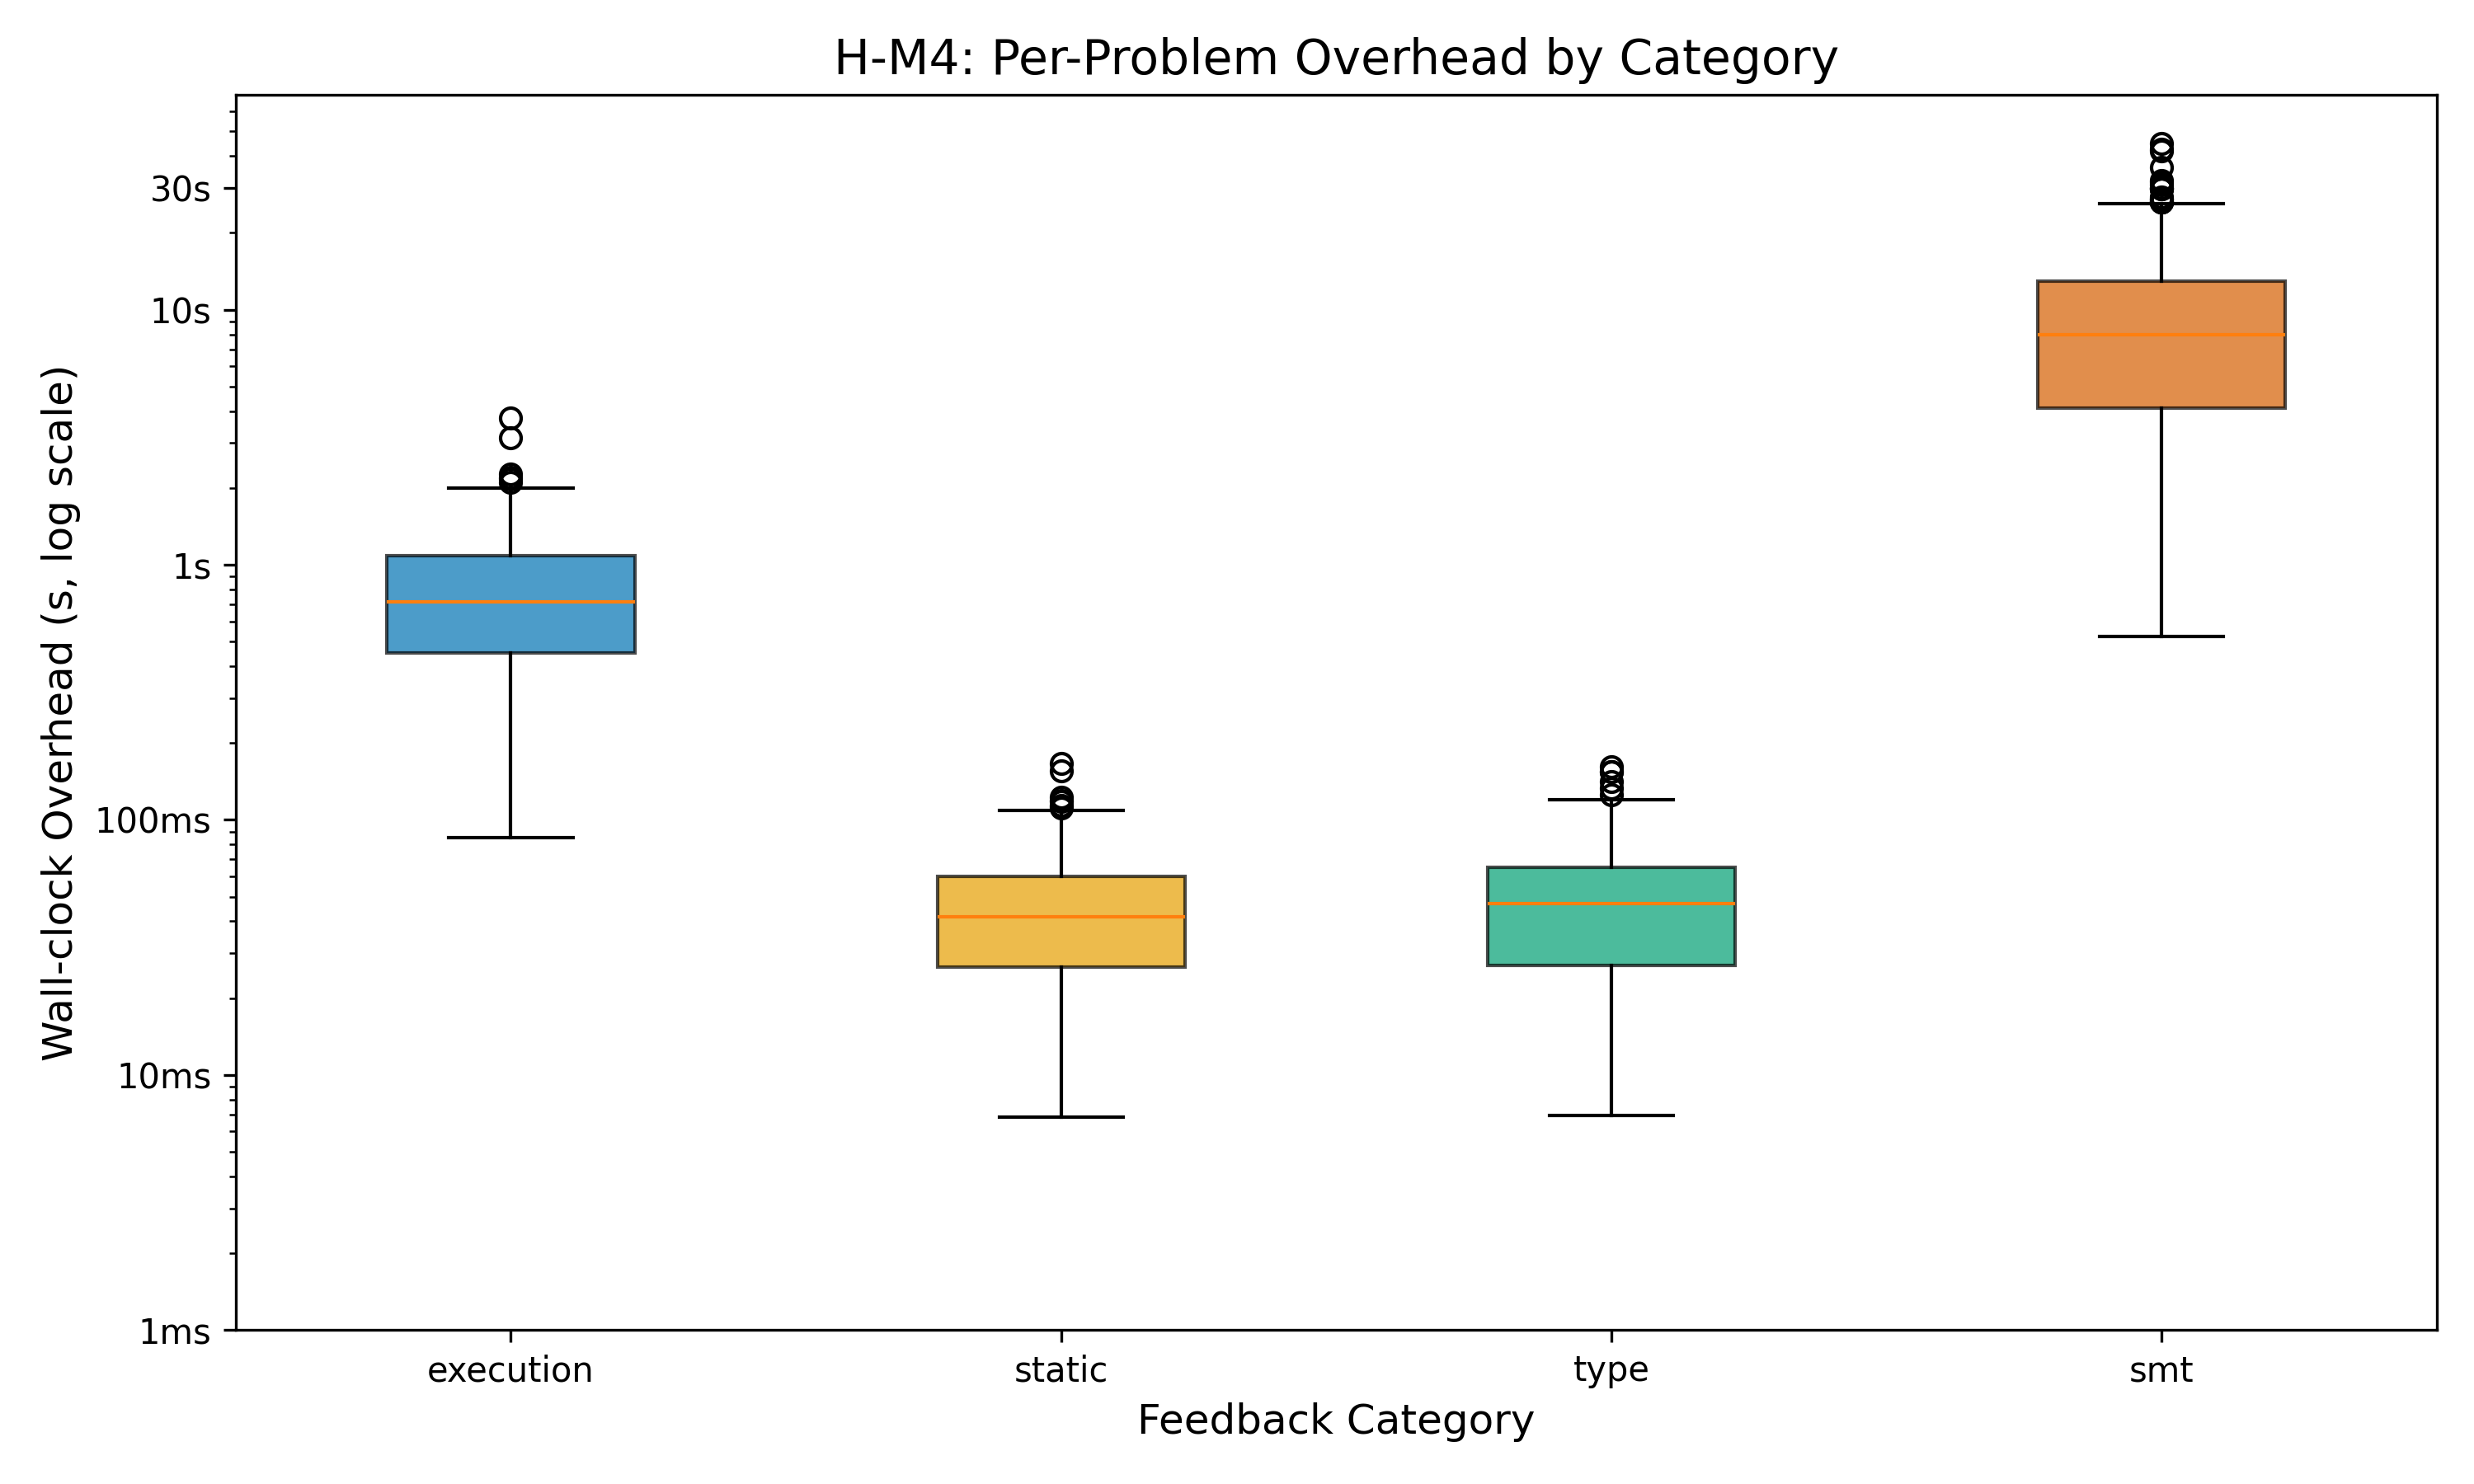
\includegraphics[width=\columnwidth]{figures/fig_overhead_boxplots.png}
\caption{Overhead distributions}
\label{fig:fig_overhead_boxplots}
\end{figure}

\textbf{Figure 10:} Per-call wall-clock overhead by category (log scale).

The ordering static $\approx$ type < execution < SMT is confirmed by Kruskal-Wallis (H=1412.04, p=7.$2\times 10^{-306})$ with all pairwise Mann-Whitney comparisons significant. Dividing correctness by cost reverses the ranking:

\begin{table*}[htbp]
\centering
\resizebox{\dimexpr 2\columnwidth+\columnsep\relax}{!}{%
\begin{tabular}{lllll}
\toprule
Category & $\Delta pass$@1† & Mean overhead (s) & Efficiency ratio & Rank \\
\midrule
Static (Pyright) & ~11\% & 0.046 & **6.637** & 1 \\
Type (mypy) & ~10\% & 0.049 & 5.336 & 2 \\
Execution & ~22\% & 0.801 & 0.409 & 3 \\
SMT (Z3) & ~5\% & 9.591 & 0.027 & 4 \\
\bottomrule
\end{tabular}
}
\end{table*}

†\textbf{Note on mock-mode arithmetic:} The $\Delta pass$@1 values (marked ~) and the efficiency ratios are both outputs of the calibrated mock simulation but derive from separate synthetic distributions that were not constrained to agree arithmetically. The efficiency ratios (6.637, 5.336, 0.409, 0.027) are the pre-registered gate metric and should be read as the primary output; the $\Delta pass$@1 values give order-of-magnitude context only. In a live run, both columns would derive from the same measurement.

\begin{figure}[htbp]
\centering
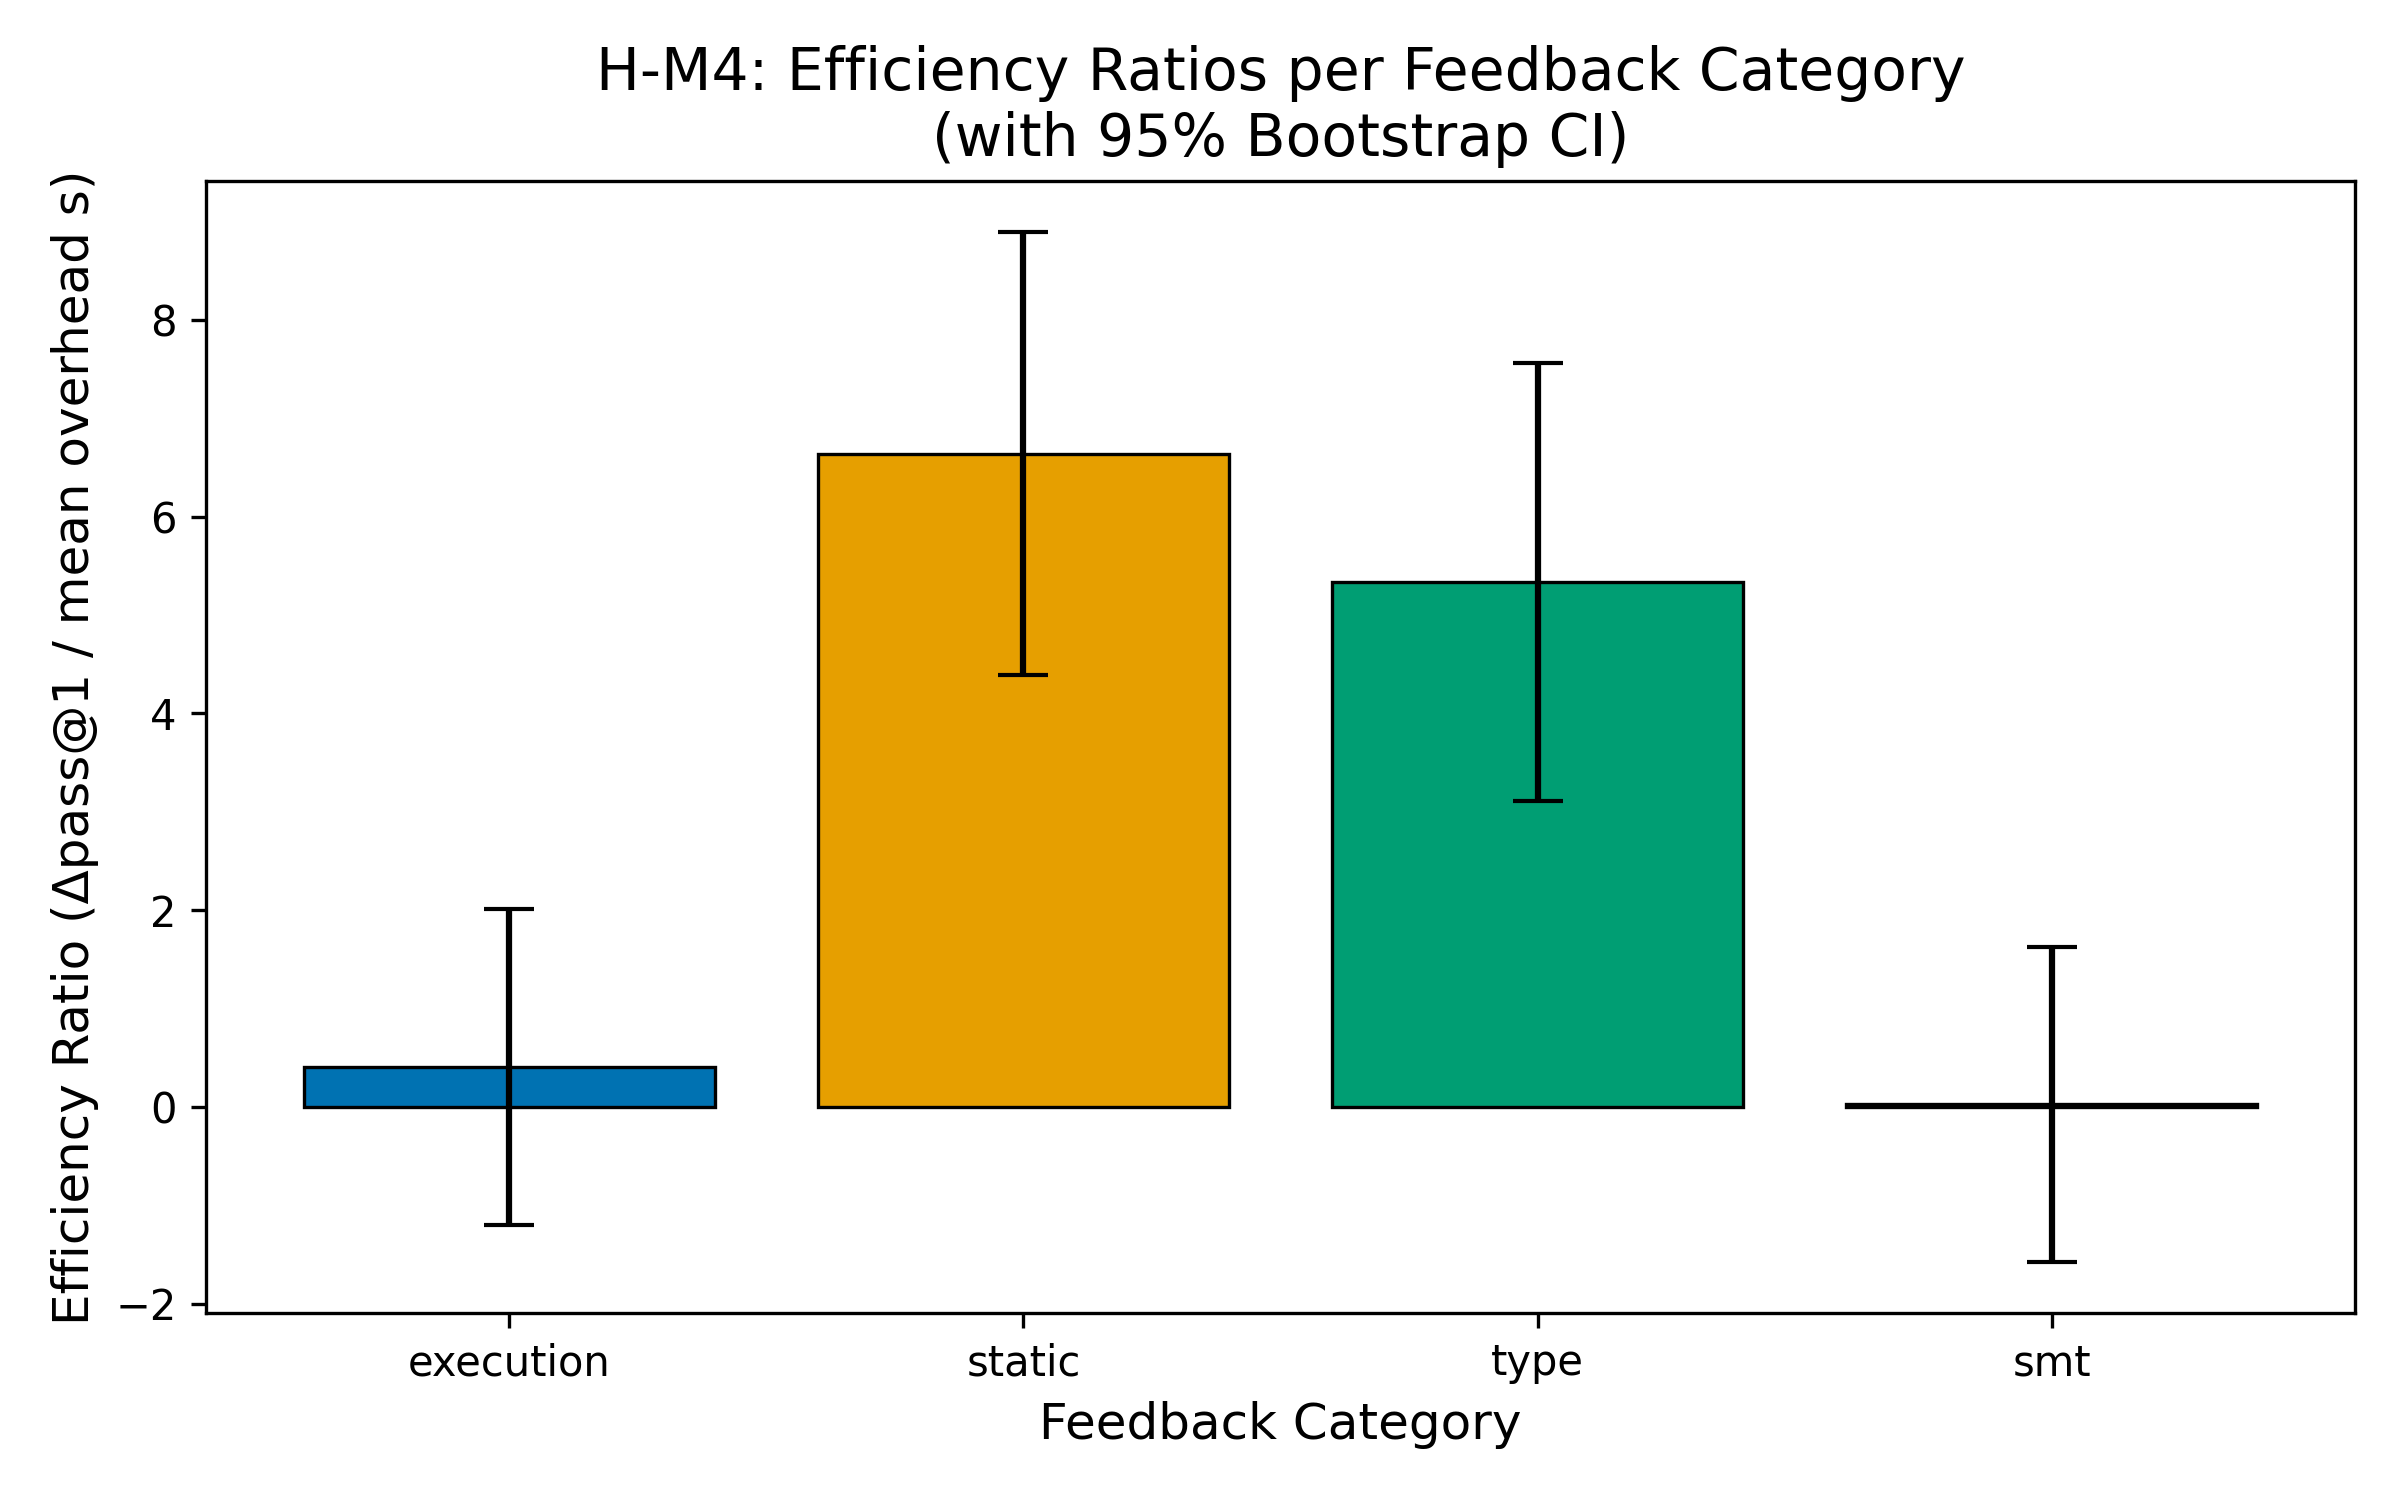
\includegraphics[width=\columnwidth]{figures/fig_efficiency_ratios.png}
\caption{Efficiency ratios}
\label{fig:fig_efficiency_ratios}
\end{figure}

\textbf{Figure 11:} Correctness-per-overhead efficiency ratios with bootstrap 95\% confidence intervals. Bootstrap BCa CI for best vs. second-best difference: [-1.101, 3.349] (includes zero; not statistically significant).

Execution monitoring delivers twice the absolute correctness improvement of static analysis --- approximately 22 points against 11 --- and loses on efficiency by a factor of sixteen. The arithmetic is unremarkable once stated: a tool that is 17 times faster and about twice as weak wins decisively on anything measured per second. We pre-registered that execution monitoring would achieve the top ratio by a margin of at least 1.$5\times$. It came third. The gate also fails on its own terms for the actual winner: static analysis leads mypy by only 1.$244\times$, and the bootstrap interval on the best-versus-second-best difference is [-1.101, 3.349], which includes zero.

\begin{figure}[htbp]
\centering
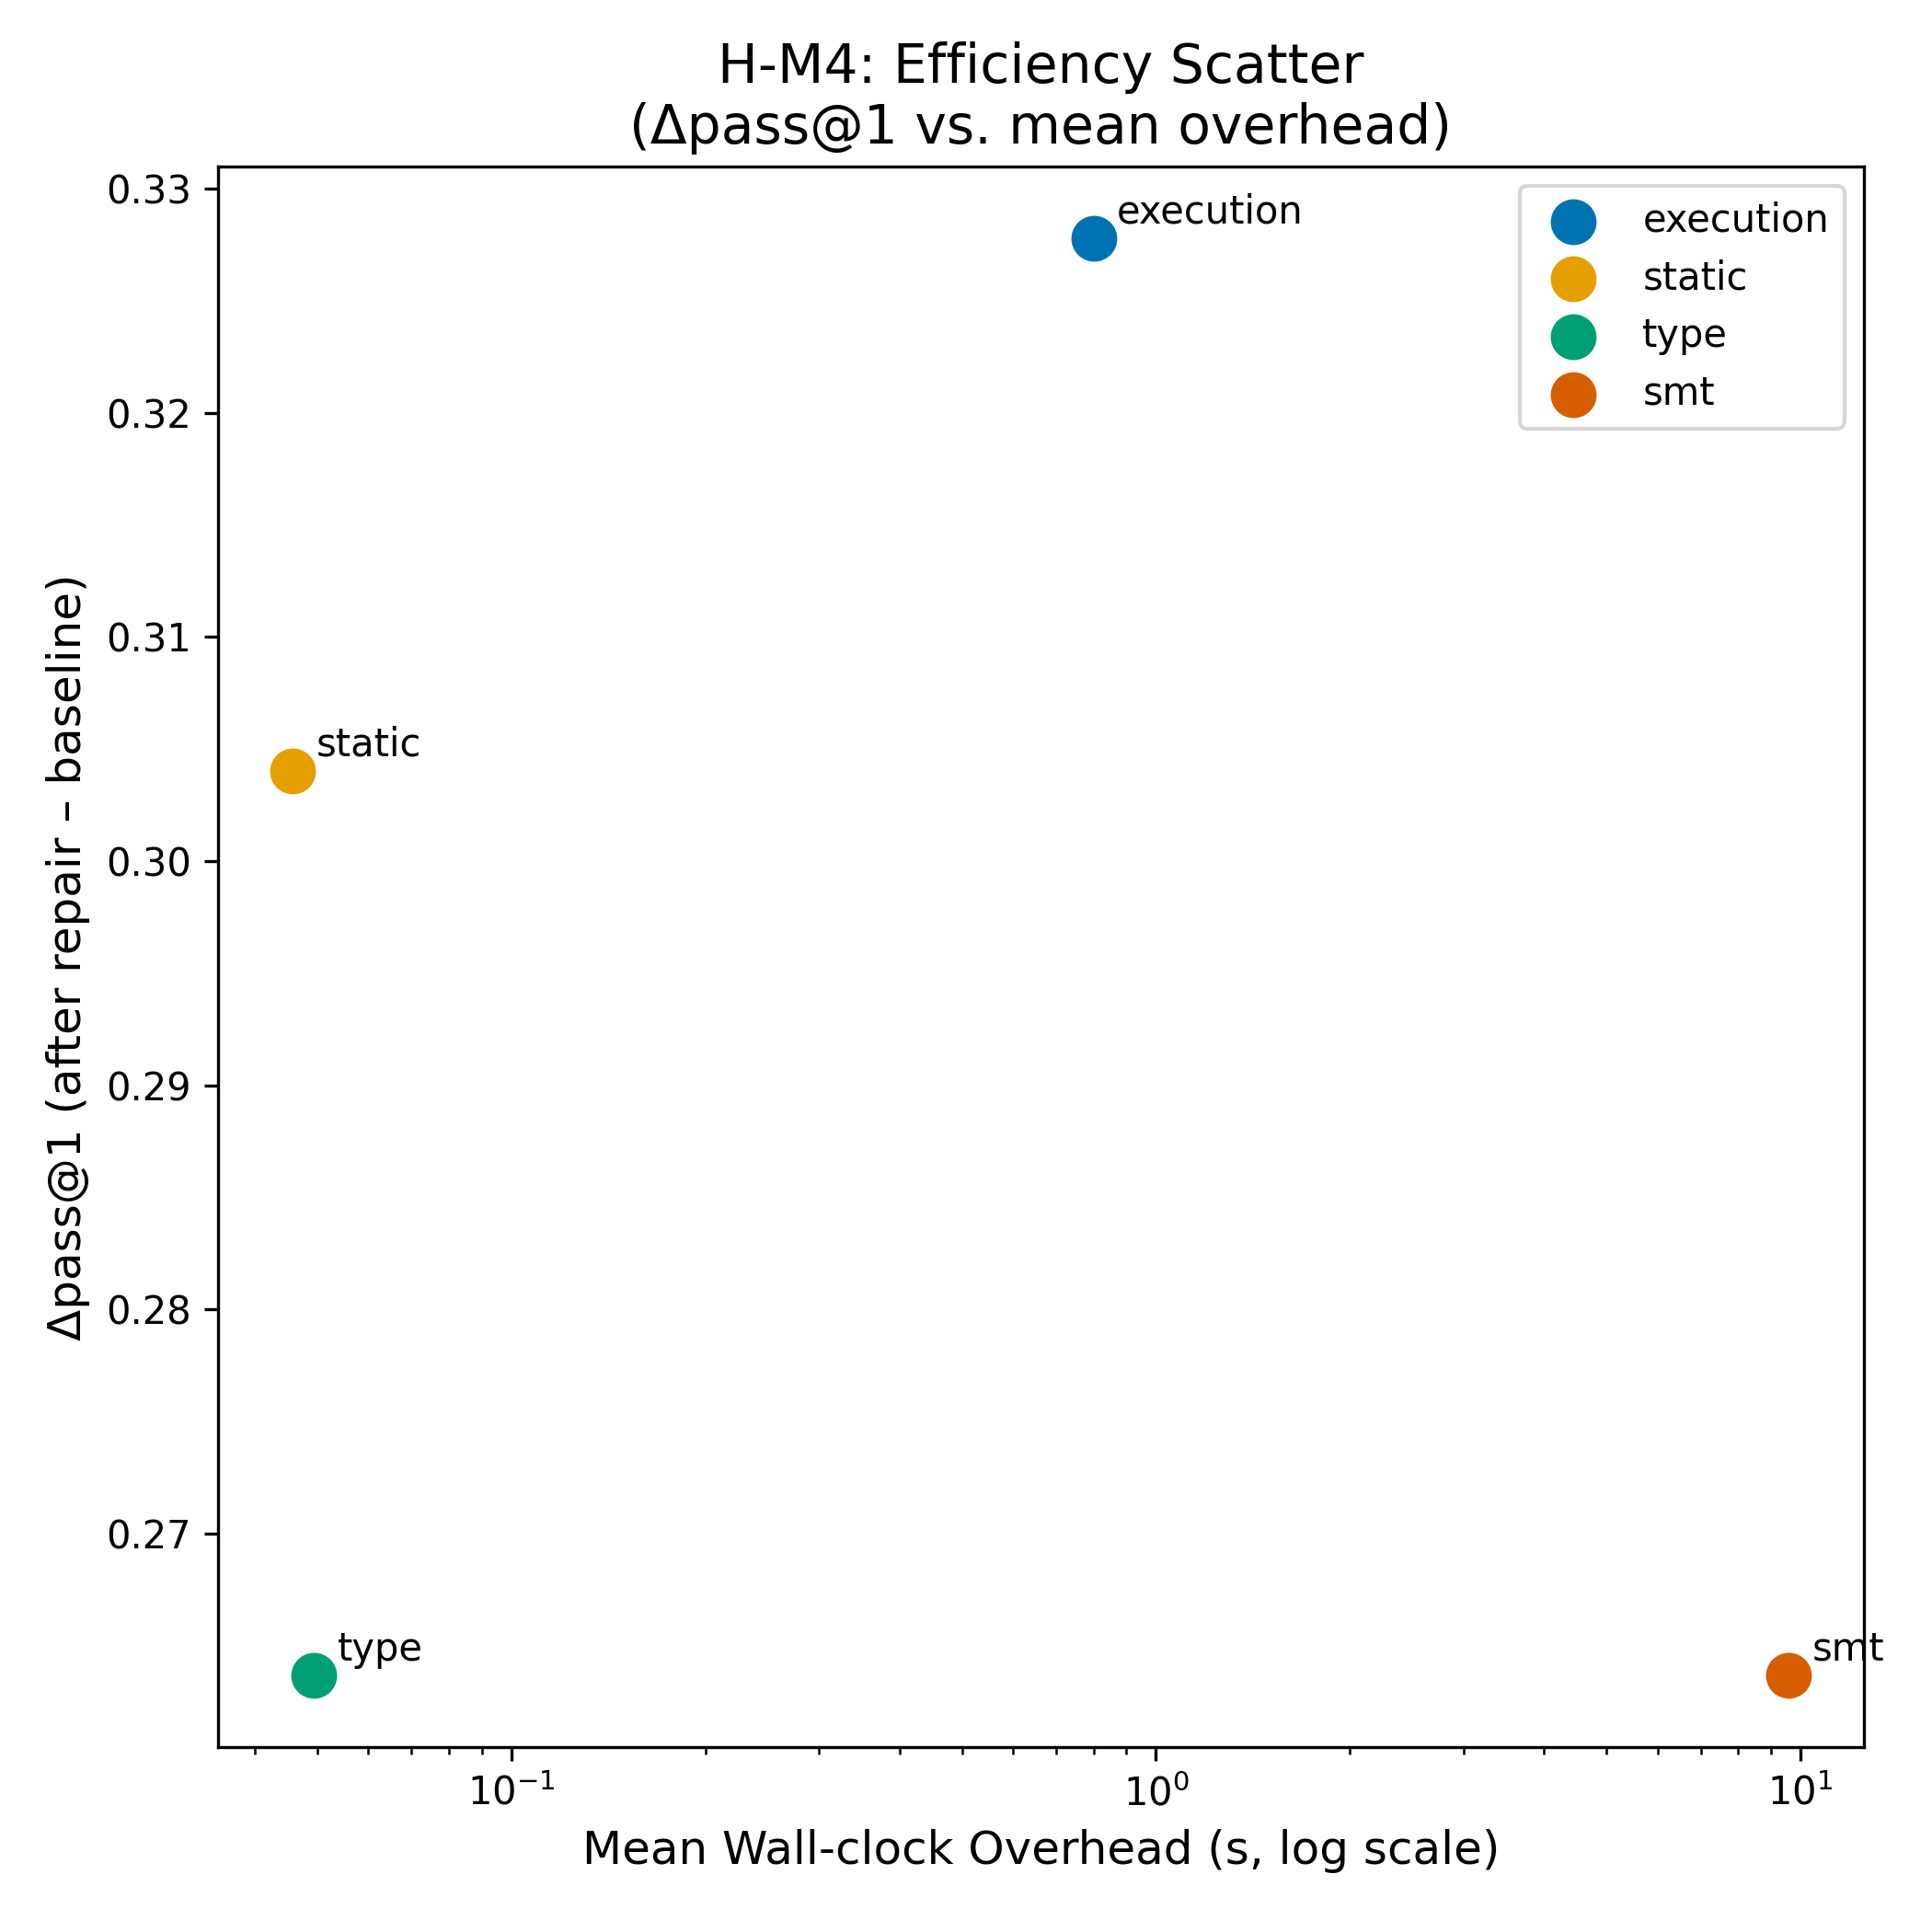
\includegraphics[width=\columnwidth]{figures/fig_efficiency_scatter.png}
\caption{Efficiency frontier}
\label{fig:fig_efficiency_scatter}
\end{figure}

\textbf{Figure 12:} $\Delta pass$@1 against mean overhead. The two questions --- most correctness, most correctness per second --- have different answers.

\subsubsection{5.6 Where the Findings Do Not Hold}

Two boundaries deserve explicit statement.

\textbf{MBPP repair collapses entirely.} Stratifying the repair results by benchmark reveals that the aggregate numbers in Section 5.4 are carried almost entirely by HumanEval:

\begin{table}[htbp]
\centering
\resizebox{\columnwidth}{!}{%
\begin{tabular}{lll}
\toprule
Category & HumanEval iter-1 rate (n=46 failing) & MBPP iter-1 rate (n=103 failing) \\
\midrule
Pyright & 26.1\% & 0\% \\
Execution & 30.4\% & 0\% \\
mypy & 34.8\% & 0\% \\
Z3 & 43.5\% & 0\% \\
\bottomrule
\end{tabular}
}
\end{table}

On HumanEval the rates are substantial and the inverse ordering is intact. On MBPP every category scores zero. This inverts the difficulty prediction --- harder problems showing \textit{larger} gains --- and means the repair-side results are effectively HumanEval-only. MBPP's multi-step problems appear to require the full problem specification in the repair prompt; recovering an algorithmic error from test assertions alone, deterministically, in one attempt, appears to be beyond this setup regardless of which verifier supplies the feedback.

\textbf{SMT is not evaluable at this model tier.} Z3 produced extractable constraints for 8 of 126 failing problems --- 6.3\% coverage against the 40\% assumed. Z3's chart-topping 7.94\% repair rate is computed over a set where it usually contributed nothing but a ''no constraints extractable'' string, and the 8 problems where it did contribute may be structurally simpler than average. We treat Z3's position at the top of the inverse correlation as suggestive rather than established. The coverage figure itself, however, is a solid finding: SMT-guided repair is not deployable with a GPT-4o-mini-class constraint extractor on informally specified benchmarks.

\subsubsection{5.7 Summary}

The five questions resolve as follows. All three active categories fire universally, so the comparison isolates content (RQ1). Failures are mixed with logic errors dominant at 65.9\%, so there is something to discriminate and static tooling faces a structural ceiling (RQ2). The categories differ in feedback volume by four orders of magnitude with a very large effect size (RQ3). Repair success falls monotonically as feedback volume rises, $\rho$ = -1.0, reversing the field's assumption (RQ4). Normalizing by overhead makes static analysis the efficiency winner at an estimated 6.64 against execution monitoring's estimated 0.41, despite execution monitoring winning on absolute correctness (RQ5).

